\documentclass[11pt]{article}

\usepackage{alltt,fullpage,graphics,color,epsfig,amsmath, amssymb}
\usepackage{hyperref}
\usepackage{boxedminipage}
\usepackage[ruled,vlined]{algorithm2e}
\usepackage{amsmath}
\usepackage{commath}
\usepackage{graphicx}
\graphicspath{ {.} }
\newcommand{\floor}[1]{\lfloor #1 \rfloor}
\newcommand{\ceil}[1]{\lceil #1 \rceil}

\title{CS 512 Assignment 2}
\author{Daniel Campos}
\date{April 25th,2021}
\begin{document}
\maketitle
\section{Problem 1}
\subsection{Short Answers}
\subsubsection{What is overfitting? What are two techniques that can mitigate this issue and explain why they handle overfitting.}
Over fitting is when a machine learn method trains to emulate the training data too closely. In other words the model has overfit its learned solution to the training data to such a degree where the performance seen on the training data is far beyond what is seen on a sample that has not been trained on. \\
One way to get around this is to always keep a portion of the dataset for validation and evaluation which you do not train on. The validation corpus can be used to tweak model performance and the evaluation portion is used as a final blind verification of model performance. This handles overfitting because it keeps a machine learning engineer honest. The validation provides a observable insight into how the model is performing on data that has not been trained on and the evaluation portion provides a complete blind evaluation which is an indication of how well this model might perform on a broader unseen data.\\
Another mechanism that can be used to mitigate overfitting is dropout. Dropout is a mechanism which each neuron in the network has some probability that it will be turned off in during the forward pass of training. This makes the network become an ensemble of sort with multiple networks working withing the larger neural network. This prevents overfitting because having ensembles of neural networks provide a broader estimation function for the training data and thus less likely to overfit. 
\subsubsection{Compare LSTM and GRU, what do they have in common and what are their differences}
LSTM's and GRU's are two different Recurrent Neural Network (RNN) architectures. RNNs are designed to process inputs in series (like time series or language data) and do so by passing a hidden state from one state to the next. GRU and LSTM have learned gates which allow them to learn what information should be encoded and what information should not be encoded in the hidden state. They are similar because they both provide methods of updating and modifying what is remembered at each iteration but they differ in their structure. GRU only feature update and reset gate while the LSTM features a update, forget and input gate. As a result LSTMs can perform better on more complicated inputs but are computationally more expensive to train/predict and they require more data to train. In general GRU's will train and infer quicker and out perform LSTM with small datasets but as the dataset grows LSTMs will outperform GRUs.
\subsection{Back Propagation}
\subsubsection{Prove the error equation for unit $U_6$ and the weight update function for the same neuron}
To calculate the degree which unit six effected the loss is equivalent to asking what effect did the output of unit 6 have on the loss. This in turn can be viewed as what effect did the out of unit 6 multiplied by its connections to units 8 and 9 and their in turn connection to unit 10, the output unit. Via the chain rule we have $\frac{\partial L}{\partial_6} = \sum_k (\frac{\partial L}{\partial_k} * \frac{\partial_k}{\partial a_6} * \frac{\partial a_6}{\partial O_6} \frac{\partial O_6}{\partial w_{i,j}})$ where $a_6$ is the output of unit six and $z_6$ is the input of unit six. Now, we address each term separately: \\
$\frac{\partial L}{\partial_k} = - \partial_k$ via the definition of $\partial$ \\
$\frac{\partial_k}{\partial a_6} = \frac{\partial}{\partial a_6} (\sum_s a_s w_{s,k}) = w_{j,k}$ as the only term in the sum that involves $a_6$ is $a_6 w_{j,k}$\\
$\frac{\partial a_6}{\partial z_6} = \frac{\partial}{\partial O_6} g(O_6)= g'(0_6) = g(O_6)(1-g(0_6)) = 0_6(1-O_6)$ where g is the sigmoid function.\\
$\frac{\partial O_6}{\partial w_{6,j}} = a_j$ since the only term that involves $w_{6,j}$ is $a_i w_{i,j}$ \\ \\
Thus combining it all $\frac{\partial L}{\partial_6} = \sum_k (-\partial_k w_{6,k} a(1-a_j) O_6)$
which we simplify to $\partial_6 = O-6(1-O_6)(\sum_k (\partial_k w_{6,k}))$ and since unit six is only connected to unit 8 and 9 we further simplify to $\partial_6 = O-6(1-O_6)(\partial_8 w_{6,8}) + \partial_9 w_{6,9})$. \\ 
The update is derived from $\frac{\partial L}{\partial w_{i,j}} = -\partial_j O_i$ which because of the gradient descent technique we add  the learning rate and get $\delta w_{i,j} = n \partial_j O_i$
\subsubsection{Derive the equation which computes the error for output unit $U_10$ for cross entropy function}
Derive the equation which computes the error for the output unit $U_10$ 
First, We know that with the cross entropy error function where D is the sample being evaluated $L= -\sum_k [t_k *log(o_k) + (1-t_k)log(1-o_k)]$. This becomes \\
$\frac{\partial L}{\partial O} = \frac{\partial}{\partial O} \sum_k [t_k log(O_k) + (1-t_k)log(1-o_k)$ . \\
$\frac{\partial L}{\partial O} = \frac{\partial}{\partial O} t log(O) - \frac{\partial}{\partial O} (1-t)log(1-O)$ . \\
$\frac{\partial L}{\partial O} = \frac{t}{O} + \frac{1-t}{1-O}$. \\
This means in turn that the $\partial_{10} = (\frac{t}{O} + \frac{1-t}{1-O})$
\subsection{2D Convolution}
\subsubsection{Compute the feature maps by applying kernel $K_1$, $K_2$ (stride = 1)}
First its important to note that because there is no specification about what form of padding to use I am not using any padding. This means that our 5x5 input becomes a 4x4 output. The feature map after applying $K_1$ can be found in table \ref{tab:conv1-k1} and the feature map after applying $K_2$ can be found in table \ref{tab:conv1-k2}. 
\begin{table}[]
\begin{tabular}{|l|l|l|l|} \hline
2 & 0 & 0 & 2 \\ \hline
0 & 0 & 2 & 0 \\ \hline
1 & 1 & 0 & 2 \\ \hline
1 & 0 & 2 & 0 \\ \hline
\end{tabular}
\caption{Resulting feature map after application of K1 on Input}
\label{tab:conv1-k1}
\end{table}
\begin{table}[]
\begin{tabular}{|l|l|l|l|} \hline
1 & 1 & 1 & 1 \\ \hline
1 & 1 & 1 & 2 \\ \hline
0 & 1 & 2 & 1 \\ \hline
1 & 1 & 1 & 2 \\ \hline
\end{tabular}
\caption{Resulting feature map after application of K2 on Input}
\label{tab:conv1-k2}
\end{table}
\subsubsection{Compute the new feature map after we apply average pooling with 2x2 filter from previous work}
Average pooling for the feature map extracted by using kernel $K_1$ can be found in table \ref{tab:conv-k1-average}, and table \ref{tab:conv1-k2-average} for the average pooling on the feature map extracted by $K_2$.
\begin{table}[]
\begin{tabular}{|l|l|} \hline
0.5 & 1 \\ \hline
0.75 & 1 \\ \hline
\end{tabular}
\caption{Average pooling for feature map using K1 on input}
\label{tab:conv-k1-average}
\end{table}
\begin{table}[]
\begin{tabular}{|l|l|} \hline
1 & 1.25 \\ \hline
0.75 & 1.5 \\ \hline
\end{tabular}
\caption{Average pooling for feature map using K2 on input}
\label{tab:conv1-k2-average}
\end{table}
\subsection{Graph Convolutional Networks}
\subsubsection{Is this task inductive learning or transductive learning}
This is inductive learning because we only see a portion of the dataset while training (the train portion: 60\%) and then we apply the learned model on dataset it has never seen before (validation/eval data portions)
The main difference is that during transductive learning, you have already encountered both the training and testing datasets when training the model. However, inductive learning encounters only the training data when training the model and applies the learned model on a dataset which it has never seen before.
\subsubsection{Implement this model and evaluate and report accuracy}
Final Loss on eval: 0.8361107707023621 and final accuracy:0.7458563535911602
\subsection{Vary the optimizer and learning rate strategies and report numbers}
First, using ADAM I vary the learning rate and training length as seen in table \ref{tab:1d}. Next, I vary the best LR (1e-1 ) and experiment with ADAM across SGD, and RMSProp finding ADAM to be the best as shown in table \ref{tab:1de}
\begin{table}[]
\begin{tabular}{|l|l|l|l|} \hline
Learning Rate & Updates & Loss & Accuracy \\ \hline
1e-1 & 100  & 0.7455894351005554 & 0.7495395948434622 \\ \hline
1e-1 & 1000  & 0.6971593499183655 & 0.7569060773480664 \\ \hline
1e-1 & 10000  & \textbf{0.6468987464904785} & \textbf{0.7992633517495397}  \\ \hline
1e-2 & 100 & 1.1029239892959595 & 0.6611418047882136 \\ \hline
1e-2 & 1000  & 0.6627088189125061 & 0.7808471454880295 \\ \hline
1e-2 & 10000  & 0.6523106694221497 & 0.7974217311233887 \\ \hline
1e-3 & 100  & 1.832948923110962 & 0.3020257826887661 \\ \hline
1e-3 & 1000  & 1.0243993997573853 & 0.6758747697974218 \\ \hline
1e-3 & 10000  & 0.6788013577461243 & 0.7808471454880295 \\ \hline
1e-4 & 100  & 1.9703178405761719 & 0.0865561694290976 \\ \hline
1e-4 & 1000  & 1.8301498889923096 & 0.3020257826887661 \\ \hline
1e-4 & 10000  & 1.0697520971298218 & 0.6666666666666667 \\ \hline
1e-5 & 100  & 1.9364348649978638 & 0.18968692449355434 \\ \hline
1e-5 & 1000  & 1.9022825956344604 & 0.3001841620626151 \\ \hline
1e-5 & 10000  & 1.8908064365386963 & 0.27808471454880296 \\ \hline
\end{tabular}
\caption{Effect of varying learning rate and training duration for GCN}
\label{tab:1d}
\end{table}

\begin{table}[]
\begin{tabular}{|l|l|l|l|} \hline
Optimizer & Updates & Loss & Accuracy \\ \hline
ADAM & 100   & 0.7455894351005554 & 0.7495395948434622 \\ \hline
ADAM & 1000   & 0.6971593499183655 & 0.7569060773480664 \\ \hline
ADAM & 10000 & \textbf{0.6468987464904785} & \textbf{0.7992633517495397} \\ \hline
SGD & 100  & 1.822108507156372 & 0.3020257826887661 \\ \hline
SGD & 1000   & 1.05472731590271 & 0.6261510128913444 \\ \hline
SGD & 10000   & 0.8426060676574707 & 0.7679558011049724 \\ \hline
RMSProp & 100  & 1.5735245943069458 & 0.40699815837937386 \\ \hline
RMSProp & 1000  & 1.5078521966934204 & 0.3830570902394107 \\ \hline
RMSProp & 10000  & 1.0892350673675537 & 0.5948434622467772 \\ \hline
\end{tabular}
\caption{Effect of varying optimizer and training duration for GCN}
\label{tab:1de}
\end{table}
\subsubsection{If the number of GCN layers increase how does the model performance change in terms of quality and efficiency}
If we increase the layers of the model we can model more complex data but do so with a computational overhead. In other words, a deeper network (more layers) is more computationally expensive to run and has a greater ability to fit the data. A deeper network can produce better accuracy but can also more easily overfit to the training data. When we add a third layer to our model our performance goes from 0.7569 to 0.784530 but the time to train goes from 1m13.765s to 1m38.955s and while the accuracy is higher for the deeper model its loss on eval is higher (0.7600502967834473 vs. 0.6616357564926147) indicating the model is overfitting.
\section{Outlier Detection}
\subsection{Short Answers}
\subsubsection{From the perspectives of outlier detection methods give two possible definitions of outliers}
One definition of an outlier would be a data point that differs so much from the expected data distribution as to make it clearly not part of the regular distribution. Another definition would be a data point which has a significant effect on the conditional probabilities learned while studying data as models will over compensate in order to fit this out of distribution sample. 
\subsection{What is the disadvantage of describing outliers as any point that is larger than the majority of values? How do we modify our definition of outliers to avoid this problem? Use examples }
This method will miss any value that is an outlier on small scale (both close to 0 and negative) and also will fail to take into account natural distribution of large values. One way to avoid this problem is to build a notion of outliers based on the distribution of the data like Grubbs test. Instead of calling extremely large values outliers we refer to values which our outside of a Gaussian distribution as outliers. 
\subsection{Implementation using $PyOD^3$}
The three methods I ran were KNN, PCA, and VAE results for runs on vowels.mat can be found in table \ref{tab:vowels} and results for runs on satimage-2 can be found in table \ref{tab:satimage}. At a broad level we see that more simple data like that of vowels, KNN performs best(and trained fastest) but as data gets harder Neural (VAE) and more complex methods (PCA) out perform. That being said neither PCA or VAE achieves the highest of scores on the satellite data as the feature space is small. 
\begin{table}[]
\begin{tabular}{|l|l|l|l|} \hline
Metric        & KNN & PCA     & VAE  \\ \hline
Precision @10 & 0.00/0.00       & 0.00/0.0    &  0.00/0.0   \\ \hline
Precision @20 & 0.00/0.00       & 0.00/0.0    &  0.00/0.0     \\ \hline
Precision @50 & \textbf{0.4/0.3571}      & 0.1429/0.105 & 0.1538/0.1136 \\ \hline
Precision @100 & \textbf{0.4/0.3571}      & 0.1429/0.1053 & 0.1538/0.1136 \\ \hline
ROC AUC Score & \textbf{0.8868/0.8955}   & 0.6336/0.6267 & 0.6372/0.6625 \\ \hline
Recall Score  & \textbf{0.8235/0.8333}   & 0.3529/0.3333 & 0.3529/0.4167 \\ \hline
\end{tabular}
\caption{Model performance on vowel dataset vowels.mat}
\label{tab:vowels}
\end{table}
\begin{table}[]
\begin{tabular}{|l|l|l|l|}\hline
Metric        & KNN & PCA     & VAE  \\ \hline
Precision @10 & 0.00/0.00       & 0.00/0.0     &  0.00/0.0   \\ \hline
Precision @20 & 0.00/0.00       & 0.00/0.0     &  0.00/0.0   \\ \hline
Precision @50 & 0.00/0.00       & 0.00/0.0     &  0.00/0.0   \\ \hline
Precision @100 & 0.00/0.00      & 0.00/0.0     &  0.00/0.0   \\ \hline
Precision @1000 & 0.0914/0.0983 & \textbf{0.1024/0.1264} & 0.0994/0.1223  \\ \hline
ROC AUC Score & 0.8666/0.8691   & 0.9331/0.9304& \textbf{0.9546/0.9252} \\ \hline
Recall Score  & 0.8182/0.8421   & 0.9545/0.9474& \textbf{1.0/0.9474} \\ \hline
\end{tabular}
\caption{Model performance on Satellite images dataset satimage-2.mat}
\label{tab:satimage}
\end{table}
\section{Gaussian Mixture Model}
\subsection{Compared with K-Means, what are the advantages and disadvantages of Gaussian mixture model}
The advantages of GMM over KNN are related to how a Gaussian models a cluster. First off, since a GMM is a probability distribution we can get confidence scores for each of these clusters which can help us decide if a data point may belong to more than one cluster. Additionally GMM can outperform KNN as they can man model more oblong clusters of data while KNN is limited to modeling circular clusters while Gaussian can become oblong shapes. This works well for data that does not have a circular distribution.  \\

The disadvantages of GMM are mostly related to the model size. There are a lot of parameters to fit which means that there are many iterations and large data is required for training. If there are few samples in the train dataset KNN may still have good performance while GMM will likely not.
\subsection{E-Step:Prove that the posterior probability of the k-th component $\gamma_{i,j}$}
First from bayes theorem $p(z_i = K| x) = \frac{p(z_i = k)p(x|z_i = k)}{\sum_{j=1}^k p(z_j = k)p(x| z_j = k)}$. \\
which since the prior probability $p(Z_i=k) = \pi_k$ we can rewrite $\gamma_{i,k} = p(z_i = K| x_i) = \frac{\pi_k  N(x_i | \mu_k , \sigma_k)}{\sum_k N(x_i| \mu_k, \sigma_k)}$ 
\subsection{M-Step:Prove that the new estimations of $\mu_k$, $\sigma_k$, $\pi_k$}
The approach we use to prove all three estimates is the same: take the derivative with respect to the variable set to 0. 
First for $u_k$: $\frac{\partial}{\partial \mu_k}= \sum_{i=1}^n \frac{\pi_k N(x_i| \mu_k, \sigma_k)}{\sum_{k=1}^K \pi_k N(x_i| \mu_k, \sigma_k)} \frac{x_i - \mu_k}{\sigma_k^2} = 0$ which given the E step can be rewritten as $\sum_{i=1}^n \gamma_{i,k}\frac{x_i - \mu_k}{\sigma_k^2} = 0 $ which can be simplified to $\frac{\sum_{i=1}^n \gamma_{i,k}x_i}{\sigma_k^2}  - \frac{\sum_{i=1}^n \gamma_{i,k}\mu_k}{\sigma_k^2} = 0 $ which then becomes $\frac{\sum_{i=1}^n \gamma_{i,k}x_i}{\sigma_k^2}  = \frac{\sum_{i=1}^n \gamma_{i,k}\mu_k}{\sigma_k^2}$, then $\frac{\sum_{i=1}^n \gamma_{i,k}x_i}{1}  = \frac{\sum_{i=1}^n \gamma_{i,k}\mu_k}{1}$, $\frac{\sum_{i=1}^n \gamma_{i,k}x_i}{\sum_{i=1}^n \gamma_{i,k}}  = \mu_k$ which is our target. \\\\
Following the same logic for $\sigma_k^2$ we first take the derivative and set to 0 we get $\frac{\partial }{\partial \sigma_k} =  (\sum_{n=1}^n \gamma_{n,k}(x_n-u_k)(x_n-u_k)) - (\sum_i \gamma_{i,k} \sigma_k^2)$ which leads to $(\sum_{n=1}^n \gamma_{n,k}(x_n-u_k)(x_n-u_k)) = (\sum_i \gamma_{i,k} \sigma_k^2)$, then $\frac{\sum_{n=1}^n \gamma_{n,k}(x_n-u_k)^2}{\sum_i \gamma_{i,k}} =  \sigma_k^2$. \\
Finally, to find the value of $\pi_k$ we must take into account mixing coefficients must sum to one. We find the maximum by using the Lagrangian multiplier and taking its derivative and setting to one. this gives $\ln p(x_i| \pi_k, \mu_k, \sigmoid_k) + \lambda (\sum_k \pi_k -1)$ which the derivative with respect to $\pi_k$ is $\frac{1}{N}*\sum_i \gamma_{i,k}$ which is our desired output
\section{Graph Connectivity and SIS model}
\subsection{Implement the Susceptible-Infected-Susceptible and graph number of people in each group}
For the initial implementation there are an average of 6876.03 infected nodes
after the convergence(200-300 iterations). The plot for susceptible and infected individuals can be found  in figure \ref{fig:sis}.
\begin{figure}
    \centering
    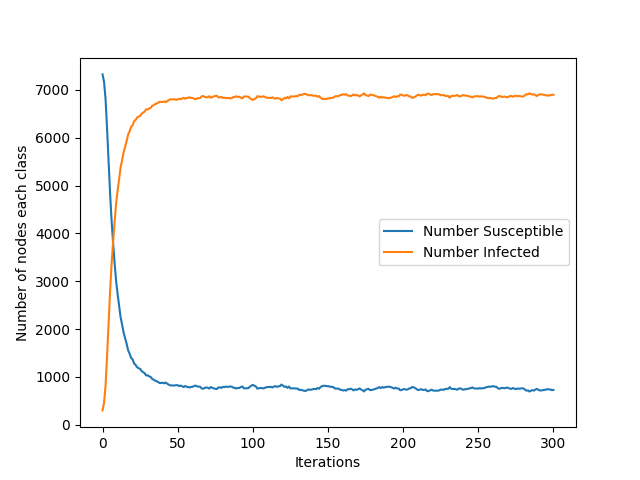
\includegraphics{Assignments/Assignment2/sis.png}
    \caption{Effect of Random Vaccination in virus propagation}
    \label{fig:sis}
\end{figure}
\subsection{Vaccination}
For random vaccination of 200 nodes the average infected nodes after convergence is 6645.46 and the plot for susceptible and infected individuals can be found  in figure \ref{fig:vacrand}.
For those with highest degree there is an average we achieve a slightly lower rate of 6215.99 and the plot for infection growth over time can be found in figure \ref{fig:highdegree}.
\begin{figure}
    \centering
    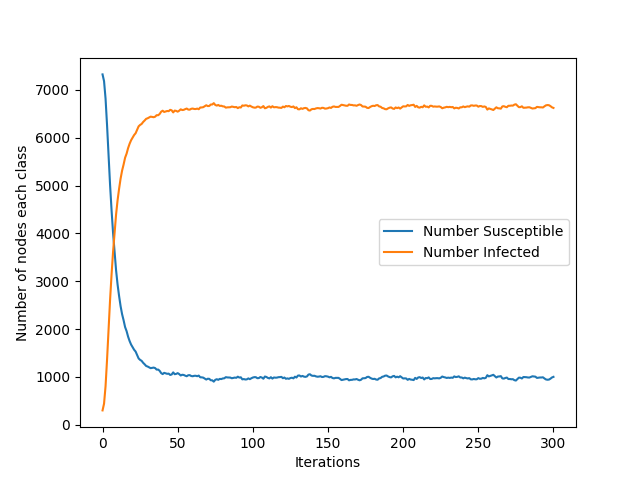
\includegraphics{Assignments/Assignment2/random-vac.png}
    \caption{Effect of Random Vaccination in virus propagation}
    \label{fig:vacrand}
\end{figure}
\begin{figure}
    \centering
    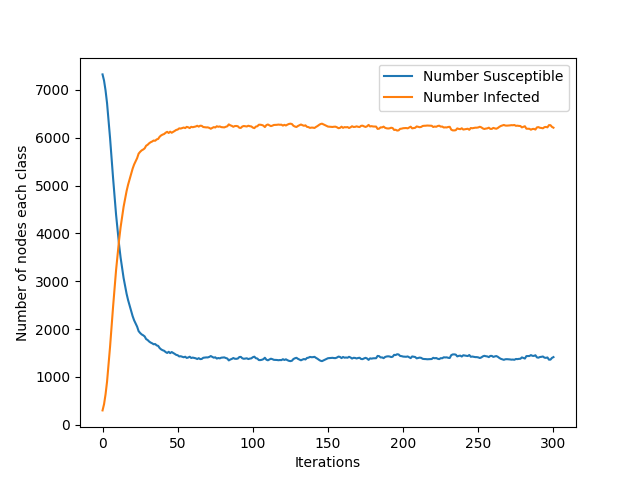
\includegraphics{Assignments/Assignment2/high-degree.png}
    \caption{Effect of High Degree Vaccination in virus propagation}
    \label{fig:highdegree}
\end{figure}
\subsection{More Vaccination}
I explore three strategies for vaccination: proximity to infected nodes at time step 0, highest connection via 2 hops, random walk. \\
For proximity to infected nodes I generate a ranking by how heavily nodes are connected to infected node. The 200 susceptible nodes with highest connection to infected nodes become vaccinated. This averages to 6342.96 infected individuals after convergence and results over time can be seen in figure \ref{fig:infection}. This method is more effective than any random method but not as effective at vaccinating the highest degree nodes. \\
For highest connection via two hop we build on the notion of highest degree nodes but take the highest number of nodes available within 2 hops (Node-Edge-Node). This averages to 6335.06 infected individuals after convergence and results over time can be seen in figure \ref{fig:2hop}. \\
For Random walk we start at an random node and vaccinate it and then walk to one of its edges and make that our new vaccination node. We continue this process until we have used all of our vaccination. This averages to 6620.56 infected individuals after convergence and results over time can be seen in figure \ref{fig:randwalk}. We can see this method is more effective than random but not by much.
\begin{figure}
    \centering
    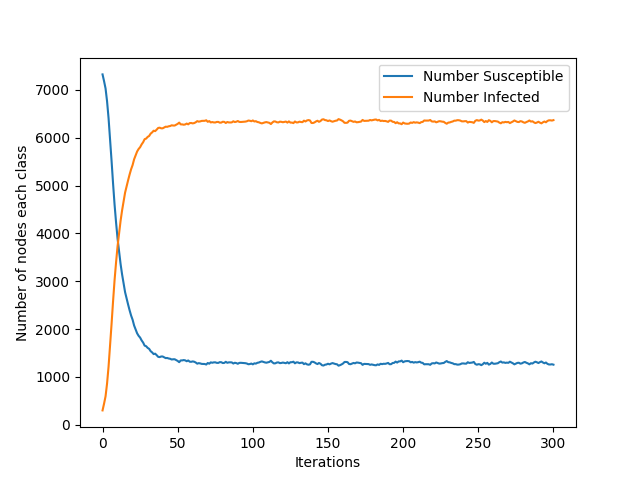
\includegraphics{Assignments/Assignment2/two_hop.png}
    \caption{Effect of Two Hop Vaccination in virus propagation}
    \label{fig:2hop}
\end{figure}
\begin{figure}
    \centering
    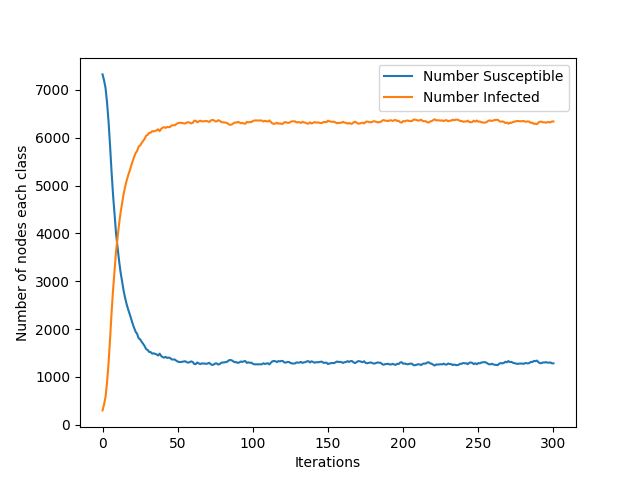
\includegraphics{Assignments/Assignment2/infection-proximity.png}
    \caption{Effect of Infection proximity Vaccination in virus propagation}
    \label{fig:infection}
\end{figure}
\begin{figure}
    \centering
    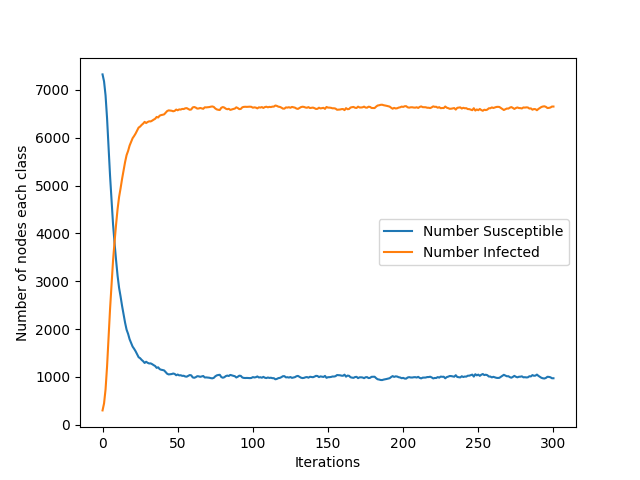
\includegraphics{Assignments/Assignment2/random-walk.png}
    \caption{Effect of Random Walk Vaccination in virus propagation}
    \label{fig:randwalk}
\end{figure}
\end{document}